\documentclass{llncs}
\usepackage{makeidx}
\usepackage{graphicx}
\usepackage{subfigure}
\usepackage[portuges]{babel}
\usepackage[utf8]{inputenc}

\begin{document}
\title{RoboIME : Team Description Paper for RoboCup 2014}
\author{
 Andre O. P. Barcelos \and
 Diego F. de Almeida \and
 Douglas K. Paixão \and
 Jan L. L. Segre \and
 Lucas O. de Lima \and
 Luis R. L. Rodrigues \and
 Naum A. F. Barreira \and
 Paulo F. F. Rosa \and
 Rafael C. Felzenszwalb \and
 Renan Gemignani \and
 Robinson C. M. B. Filho \and
 Stefano H. Rodrigues \and
 Thiago A. N. do Amaral \and
 Vitor H. F. Betio \and
 Vitor L. H. Ferreira \and
 Victor Bramigk
}

\institute{Seção de Engenharia de Computação \\ Instituto Militar de Engenharia (IME) \\ Praça General Tibúrcio, 80 - Praia Vermelha, Urca \\ Rio de Janeiro - RJ - Brazil \\ \email{roboime@googlegroups.com}}
\maketitle
%
\begin{abstract}
This paper describes the electronic, mechanical and software designs developed by RoboIME Team in order to join RoboCup 2014. All designs are in agreement with the rules of Small Size League 2014. This is the second RoboIME participation in a world level RoboCup event, although the team was already challenged third in Brazilian competitions.
\end{abstract}

\section{Introduction}
RoboIME is a small-size league soccer robot team from IME, Rio de Janeiro, Brazil. This is only the third time the team is taking part in competitions. The main result was in 2012 when the team achieved second place in Latin American Robotics Competition.

All students that work in this project are members of the Laboratório de Robótica e Inteligência Computacional at IME. The previous studies \cite{alexandre}\cite{marco} provided the basis for the current structure of software and hardware team's. This paper describe the computer, electronic and mechanical design.

\section{Software System}

The software systems consist of three projects: pyroboime (AI), ssl-webclient (graphical client), grSim (simulator).

\subsection{AI}

The AI, pyroboime, is based on the STP (Skill-Tactic-Play) architecture and implemented in python.
It has the following components: interface with the ssl-vision, ssl-refbox and grSim, it also has a built-in communication module for the radio transmitter system.

The STP is a three tier architecture where the lowest level, skills, enables the low level manipulations on a single robot.
The middle layer, tactics, makes use of the skill layer to execute higher level behaviour, possibly enabling coopration, but still acting on a single robot.
The upper layer, plays, coordinates the tactics associated to each robot in order to maximize performance, each play is implemented to behave according to specific states: stop, halt, indirect kicks and normal play.
A higher level layer implmented as a play switches between other plays based on the current referee state.

The interface is structured as a filter stack which connects the AI to a flexible collection of updaters (which receive state information) and commanders (which deliver commands to the robots, in both the simulated and real environments).
It abstracts the external environment where the game is played from the AI.
Among the filters in said stack is a Kalman filter that reduces the noise comming from the updater data.

The built-in radio trasmitter system interfaces with libusb to control the transmitter hardware, which is connected via USB.

\begin{figure}[thpb]
     \centering
     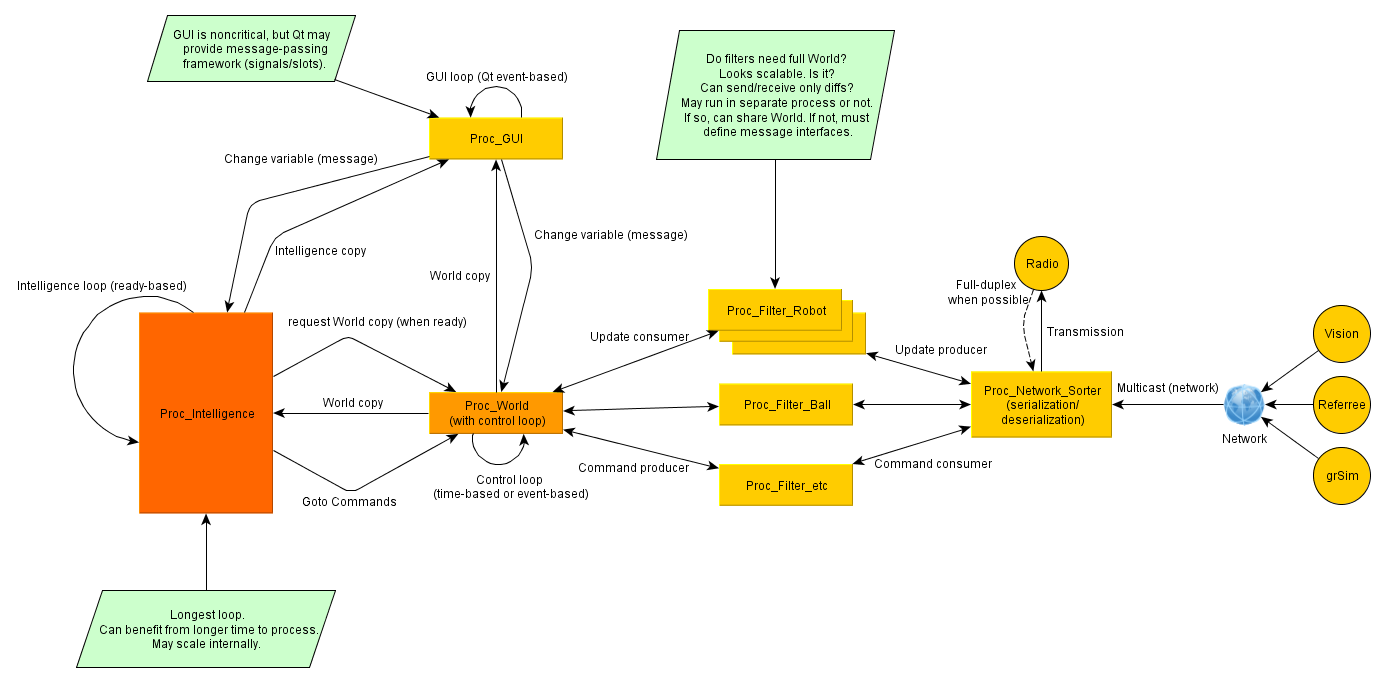
\includegraphics[width=15cm]{img/software-model.png}
     \caption{Block diagram of the AI software}
     \label{fluxogramSoftware}
\end{figure}

\subsection{Support systems}

The graphical client, ssl-webclient, is a Web interface implemented in nodejs using WebSockets, HTML5, SVG and ZeroMQ.
It has the following functionality: displaying and altering the AI state, broadcasting games through the internet and playing log files.

Lastly the simulator, grSim, originally developed by Parsian Robotic, was customized to fit our needs.
It provides the following functionality: simulating the game environment and exposing an ssl-vision compliant protocol.

\subsection{Source}

All of the projects above have been open sourced with GPL-like license, with the main difference being that a derived work used on a competition must have its source released by the next edition of that competition. The sources of those projects are available on the team's github page: \url{http://github.com/roboime/}.

\section{Electronic Project}
RoboIME electronics consist of seven boards: (a) the Main board, responsible for communication between the other boards; (b) the Stamp board,  responsible  for the embedded computation; (c) the Kicker board, responsible for maintaining the high voltage to activate the kick shoot; (d) four motor controller board which are responsible for robot's motion control. These boards are described in details in this section.

\subsection{Main Board}
The Main Board features a socket to plugin the boards: kick's sensor, dribble's motor, four wheel's motor, four encoders and the power supply. There is a RFM12b SMD embedded which is a wireless transceiver operating in the 434 MHz band, set as up to 115.2 kbps, fully in agreement with with FCC and ETSI regulations.

The communication protocol used between the Stamp Board and the transceiver was Serial Peripheral Interface Bus (SPI), that  is a synchronous serial data link standard that operates in full duplex mode.

\subsection{Stamp Board}
This board is responsible  for performing all the logic functions. It is like a brain of the electronic system. There is a embedded micro-controller STM32F407, that has ARM Cortex M4 as main CPU, 1 MB Flash, 192 KB RAM memory, working in 168 MHz, that was programmed with C language using the  interface development CoIDE and Eclipse IDE.
%vide http://www.st.com/st-web-ui/static/active/en/resource/sales_and_marketing/promotional_material/brochure/brstm32f4.pdf

\subsection{Kicker Board}
This board is responsible for controlling the kick strength. There are two kinds of kick,
the kick shoot and the high kick. Two capacitors of 2200 $\mu$F, 200 V are used store the
voltage in a boost circuit. The charge is discharged in a solenoid and depending on the PWM
signal the kick device is activated, it is possible to control the kick velocity.

%include image of high kick

\subsection{Motor Controller Board}
The idea of the RoboIME electronic is to modularize the electronic project. So, there
is controller module board for each wheel's motor. If one of them burns out, it is
possible to change quickly. Each board has two TC4427 (MOSFET driver) and two
IRF7319 (half H bridge). These ICs create a H-bridge, allowing velocity control in
both directions.

\section{Mechanical Project}

%%%%%%%%%%%%%%%%%%%%%%%%%%%COLOCAR OS DADOS REAIS DO NOSSO ROB              %%%%%%%%%%%%%%%%%%%%%%%%
In compliance with the SSL rules, the height of the robot is 148 mm, the maximum
percentage of ball coverage is 15\% and the maximum projection of the robot on the ground is 175 mm.
%%%%%%%%%%%%%%%%%%%%%%%%%%%COLOCAR OS DADOS REAIS DO NOSSO ROB              %%%%%%%%%%%%%%%%%%%%%%%%

With the aid of CAD software (Computer Aided Design) and CAM (Computer Aided
Manufacturing) a new robot has been developed. Figure \ref{mec} shows mechanical
3D view and real view of the robot. Shelf had been used allows omnidirectional
movement and has a greater torque that couples the fourth motors (one for each
wheel) for the movement.

\begin{figure}[thpb]
	\centering
	\subfigure[]{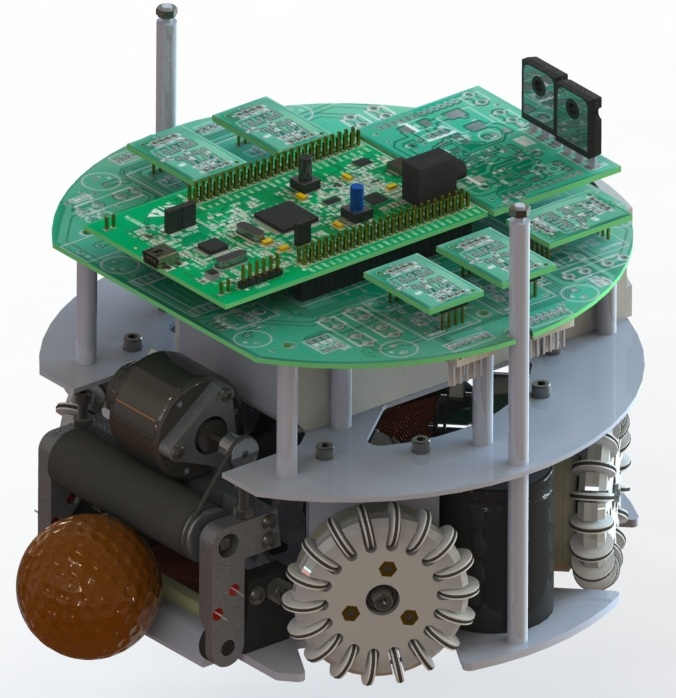
\includegraphics[width = 0.425 \textwidth]{img/cad.jpg}}
	\subfigure[]{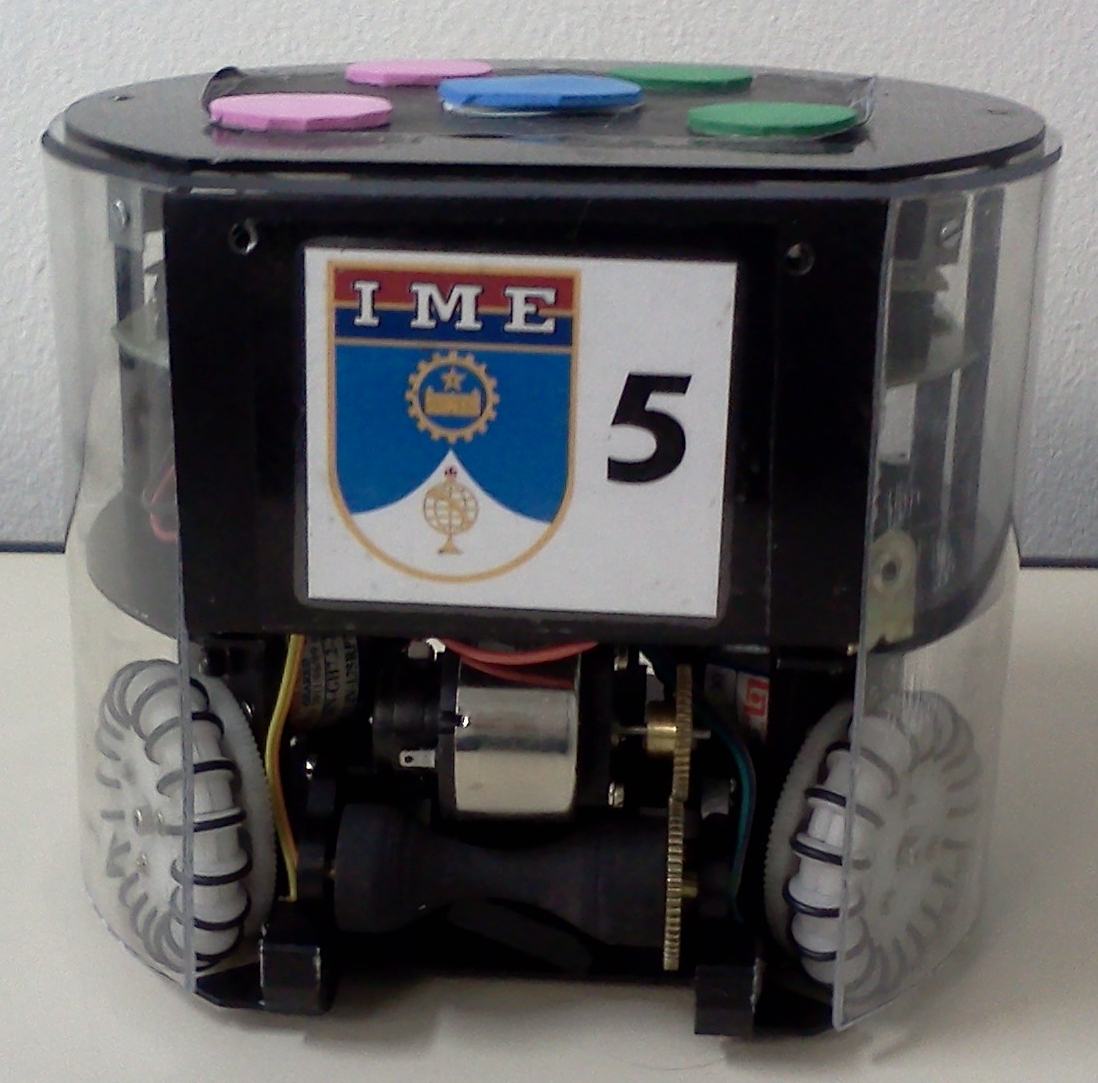
\includegraphics[width = 0.4 \textwidth]{img/robo.jpeg}}
	\caption{(a) Mechanical 3D model view. (b) Robot view.}
	\label{mec}
\end{figure}

The changes in the original design of the model provides a lower weight to
the robot, such as: changing the steel shaft by a shaft of high-strength
aluminium wheels and replacement of aluminium by plastic wheels Polytec
1000. This new design also enables more devices to be shipped. It presents
a diameter of 175 mm and an upper base with holes which give versatility
to the coupling. The fairing of the robot was made from polyvinyl plates.

\section{Final Comments}
The development of the Robocup 2014 mechanical project was concluded last year,
based on the one we created for Brazilian Robotics Competition 2012. The six
robots have already been manufactured, with only a few parts still needing rework.

Some electronic prototypes were made, yet stabilizing efforts are still ongoing.
Problems with kicker board due to hight welding temperature were observed. The solution
was to use a welding temperature below 260$^o$C.

The five modules of the AI system have already been implemented but they still
need to be brought to perfection.

Research in machine learning was started last year to predict enemy behaviour,
but an implementation is not planned for Robocup 2014.

To the June competition, following goals are being sought:
rework the remaining parts on the mechanical project such as making improvements on the coiling of the solenoid coil;
stabilize the electronic project, including robot feedback and
conclude the implementation of planning algorithms to be used in support decision making.

\section*{Acknowledgements}
This research was partially supported by Fundação Carlos Chagas Filho de Amparo a Pesquisa do Estado do Rio de Janeiro -FAPERJ(grant E-26/111.362/2012); Fundação Ricardo Franco (FRF) and Fabrica de Material de Comunicação e Eletrônica (FMCE/IMBEL). The team also acknowledges the assistance of Mr. Carlos Beckhauser from FMCE.



\begin{thebibliography}{7}
%%%%%%%%%%%%%%%%%%%%%%

\bibitem{alexandre}
Alexandre Tadeu Rossini da Silva:
Comportamento social cooperativo na realização de tarefas em
ambientes dinâmicos e competitivos.
Instituto Militar de Engenharia, Rio de Janeiro (2006)

\bibitem{tdp}
Madeira, B.~E., de~Almeida, D.~F., de~C.~Maia~Jr., E., Rodrigues, L. R.~L.,
  Rosa, P. F.~F., Rodrigues, S.~H., and do~Amaral, T. A.~N.:
RoboIME: Team Description Paper for RoboCup 2012.

\bibitem{STP}
B. Browning and J. Bruce and M. Bowling and M. Veloso:
STP: Skills, tactics and plays for multi-robot control in adversarial environments
Carnegie Mellon University, Pittsburgh, PA (2004)

\bibitem{CPA}
Khatib, O.:
Real-Time Obstacle Avoidance for Manipulators and Mobile Robots.
In International Journal of Robotics Research, vol. 5, no. 1, p. 90-98 (1986)

\bibitem{marco}
Marco Antonio Firmino de Sousa:
Uma Plataforma para Cooperação Autónoma de Múltiplos Robôs
Instituto Militar de Engenharia, Rio de Janeiro (2008)

\bibitem{minimax} Russell, Stuart J.; Norvig, Peter:
Artificial Intelligence: A Modern Approach (2nd ed.)
Upper Saddle River, New Jersey: Prentice Hall, pp. 163-171 (2003)

\bibitem{zickler}
Stefan Zickler:
Physics-Based Robot Motion Planning in Dynamic Multi-Body Environments
Carnegie Mellon University, Pittsburgh, PA (2010)

\bibitem {ekf}
Welch, G. and Bishop, G.:
An introduction to the Kalman filter. Technical Report TR 95-041, Department of
Computer Science, University of North Carolina (2001)


%\bibitem{simCamera}
%Stefan Zickler, Olivier Michel:
%SSL-vision Webots integration
%http://youtu.be/sRAVELC8jKM, 26/02/2012


\end{thebibliography}

\end{document}
